% Options for packages loaded elsewhere
% Options for packages loaded elsewhere
\PassOptionsToPackage{unicode}{hyperref}
\PassOptionsToPackage{hyphens}{url}
\PassOptionsToPackage{dvipsnames,svgnames,x11names}{xcolor}
%
\documentclass[
]{agujournal2019}
\usepackage{xcolor}
\usepackage{amsmath,amssymb}
\setcounter{secnumdepth}{5}
\usepackage{iftex}
\ifPDFTeX
  \usepackage[T1]{fontenc}
  \usepackage[utf8]{inputenc}
  \usepackage{textcomp} % provide euro and other symbols
\else % if luatex or xetex
  \usepackage{unicode-math} % this also loads fontspec
  \defaultfontfeatures{Scale=MatchLowercase}
  \defaultfontfeatures[\rmfamily]{Ligatures=TeX,Scale=1}
\fi
\usepackage{lmodern}
\ifPDFTeX\else
  % xetex/luatex font selection
\fi
% Use upquote if available, for straight quotes in verbatim environments
\IfFileExists{upquote.sty}{\usepackage{upquote}}{}
\IfFileExists{microtype.sty}{% use microtype if available
  \usepackage[]{microtype}
  \UseMicrotypeSet[protrusion]{basicmath} % disable protrusion for tt fonts
}{}
\makeatletter
\@ifundefined{KOMAClassName}{% if non-KOMA class
  \IfFileExists{parskip.sty}{%
    \usepackage{parskip}
  }{% else
    \setlength{\parindent}{0pt}
    \setlength{\parskip}{6pt plus 2pt minus 1pt}}
}{% if KOMA class
  \KOMAoptions{parskip=half}}
\makeatother
% Make \paragraph and \subparagraph free-standing
\makeatletter
\ifx\paragraph\undefined\else
  \let\oldparagraph\paragraph
  \renewcommand{\paragraph}{
    \@ifstar
      \xxxParagraphStar
      \xxxParagraphNoStar
  }
  \newcommand{\xxxParagraphStar}[1]{\oldparagraph*{#1}\mbox{}}
  \newcommand{\xxxParagraphNoStar}[1]{\oldparagraph{#1}\mbox{}}
\fi
\ifx\subparagraph\undefined\else
  \let\oldsubparagraph\subparagraph
  \renewcommand{\subparagraph}{
    \@ifstar
      \xxxSubParagraphStar
      \xxxSubParagraphNoStar
  }
  \newcommand{\xxxSubParagraphStar}[1]{\oldsubparagraph*{#1}\mbox{}}
  \newcommand{\xxxSubParagraphNoStar}[1]{\oldsubparagraph{#1}\mbox{}}
\fi
\makeatother


\usepackage{longtable,booktabs,array}
\usepackage{calc} % for calculating minipage widths
% Correct order of tables after \paragraph or \subparagraph
\usepackage{etoolbox}
\makeatletter
\patchcmd\longtable{\par}{\if@noskipsec\mbox{}\fi\par}{}{}
\makeatother
% Allow footnotes in longtable head/foot
\IfFileExists{footnotehyper.sty}{\usepackage{footnotehyper}}{\usepackage{footnote}}
\makesavenoteenv{longtable}
\usepackage{graphicx}
\makeatletter
\newsavebox\pandoc@box
\newcommand*\pandocbounded[1]{% scales image to fit in text height/width
  \sbox\pandoc@box{#1}%
  \Gscale@div\@tempa{\textheight}{\dimexpr\ht\pandoc@box+\dp\pandoc@box\relax}%
  \Gscale@div\@tempb{\linewidth}{\wd\pandoc@box}%
  \ifdim\@tempb\p@<\@tempa\p@\let\@tempa\@tempb\fi% select the smaller of both
  \ifdim\@tempa\p@<\p@\scalebox{\@tempa}{\usebox\pandoc@box}%
  \else\usebox{\pandoc@box}%
  \fi%
}
% Set default figure placement to htbp
\def\fps@figure{htbp}
\makeatother


% definitions for citeproc citations
\NewDocumentCommand\citeproctext{}{}
\NewDocumentCommand\citeproc{mm}{%
  \begingroup\def\citeproctext{#2}\cite{#1}\endgroup}
\makeatletter
 % allow citations to break across lines
 \let\@cite@ofmt\@firstofone
 % avoid brackets around text for \cite:
 \def\@biblabel#1{}
 \def\@cite#1#2{{#1\if@tempswa , #2\fi}}
\makeatother
\newlength{\cslhangindent}
\setlength{\cslhangindent}{1.5em}
\newlength{\csllabelwidth}
\setlength{\csllabelwidth}{3em}
\newenvironment{CSLReferences}[2] % #1 hanging-indent, #2 entry-spacing
 {\begin{list}{}{%
  \setlength{\itemindent}{0pt}
  \setlength{\leftmargin}{0pt}
  \setlength{\parsep}{0pt}
  % turn on hanging indent if param 1 is 1
  \ifodd #1
   \setlength{\leftmargin}{\cslhangindent}
   \setlength{\itemindent}{-1\cslhangindent}
  \fi
  % set entry spacing
  \setlength{\itemsep}{#2\baselineskip}}}
 {\end{list}}
\usepackage{calc}
\newcommand{\CSLBlock}[1]{\hfill\break\parbox[t]{\linewidth}{\strut\ignorespaces#1\strut}}
\newcommand{\CSLLeftMargin}[1]{\parbox[t]{\csllabelwidth}{\strut#1\strut}}
\newcommand{\CSLRightInline}[1]{\parbox[t]{\linewidth - \csllabelwidth}{\strut#1\strut}}
\newcommand{\CSLIndent}[1]{\hspace{\cslhangindent}#1}



\setlength{\emergencystretch}{3em} % prevent overfull lines

\providecommand{\tightlist}{%
  \setlength{\itemsep}{0pt}\setlength{\parskip}{0pt}}



 


\usepackage{url} %this package should fix any errors with URLs in refs.
\usepackage{lineno}
\usepackage[inline]{trackchanges} %for better track changes. finalnew option will compile document with changes incorporated.
\usepackage{soul}
\linenumbers
\makeatletter
\@ifpackageloaded{caption}{}{\usepackage{caption}}
\AtBeginDocument{%
\ifdefined\contentsname
  \renewcommand*\contentsname{Table of contents}
\else
  \newcommand\contentsname{Table of contents}
\fi
\ifdefined\listfigurename
  \renewcommand*\listfigurename{List of Figures}
\else
  \newcommand\listfigurename{List of Figures}
\fi
\ifdefined\listtablename
  \renewcommand*\listtablename{List of Tables}
\else
  \newcommand\listtablename{List of Tables}
\fi
\ifdefined\figurename
  \renewcommand*\figurename{Figure}
\else
  \newcommand\figurename{Figure}
\fi
\ifdefined\tablename
  \renewcommand*\tablename{Table}
\else
  \newcommand\tablename{Table}
\fi
}
\@ifpackageloaded{float}{}{\usepackage{float}}
\floatstyle{ruled}
\@ifundefined{c@chapter}{\newfloat{codelisting}{h}{lop}}{\newfloat{codelisting}{h}{lop}[chapter]}
\floatname{codelisting}{Listing}
\newcommand*\listoflistings{\listof{codelisting}{List of Listings}}
\makeatother
\makeatletter
\makeatother
\makeatletter
\@ifpackageloaded{caption}{}{\usepackage{caption}}
\@ifpackageloaded{subcaption}{}{\usepackage{subcaption}}
\makeatother
\usepackage{bookmark}
\IfFileExists{xurl.sty}{\usepackage{xurl}}{} % add URL line breaks if available
\urlstyle{same}
\hypersetup{
  pdftitle={Quantifying Climate Disequilibrium and Committed Retreat of Greenland's Peripheral Glaciers Using Landsat-Derived Accumulation Area Ratios},
  pdfauthor={Travis Zalesky; Miguel Arteaga; Alli N Cramer; Jiwei Li; Laura Larocca},
  pdfkeywords={Glacier Mass Balance, Accumulation Area
Ratio, Landsat, Remote Sensing, Machine Learning, Landcover
Classification, AGU 2026},
  colorlinks=true,
  linkcolor={blue},
  filecolor={Maroon},
  citecolor={Blue},
  urlcolor={Blue},
  pdfcreator={LaTeX via pandoc}}



\draftfalse

\begin{document}
\title{Quantifying Climate Disequilibrium and Committed Retreat of
Greenland's Peripheral Glaciers Using Landsat-Derived Accumulation Area
Ratios}

\authors{Travis Zalesky\affil{1}, Miguel Arteaga\affil{1}, Alli N
Cramer\affil{2}, Jiwei Li\affil{1}, Laura Larocca\affil{1}}
\affiliation{1}{Arizona State University, School of Ocean
Futures, }\affiliation{2}{Arizona State University, School of
Mathematical and Natural Sciences, }
\correspondingauthor{Travis Zalesky}{tzalesky@asu.edu}







\section{Methods}\label{sec-methods}

\subsection{Model Training and Validation}\label{sec-training}

Machine learning (ML) classification of Landsat images was based on a
modified version of methods published by Aberle et al. (2025). Initial
training data (labeled points and images) was acquired courtesy of
Aberle et al.~for 4 USGS Benchmark glaciers (Gulkana, South Cascade,
Sperry, and Wolverine) across 7 Landsat images, for a total of 8,162
training points. These labeled training points were augmented with an
additional 2,650 training points within Greenland, for a combined total
of 10,812 training points. For Greenland training data, two locations
were chosen, Mittivakkat glacier in south-east Greenland, and a heavily
glaciated rocky peninsula in west-central Greenland (72°N, 54°W; north
of Disko Island). Additionally, the ``cloud'' class was added to the
list of 5 landcover types from Aberle et al. (2025), bringing the total
number of land cover classifications to 6, ``cloud'', ``ice/firn'',
``rock'', ``shadowed snow'', ``snow'', and ``water''.

Surface reflectance Landsat 8 \& 9 images were acquired for each of
these training locations/dates via Google Earth Engine (GEE). Where
multiple Landsat images overlapped within a 1-hour window for a single
glacier (i.e.~successive Landsat rows), images were merged using a
median pixel value, as described by Aberle et al. (2025). For each
training image five spectral indices were calculated to aid in image
classification; Normalized Difference Snow Index (NDSI),
Normalized Difference Glacier Index (NDGI),
Normalized Difference Water Index (NDWI),
Normalized SWIR Difference Soil-moisture (NSDS), and
Normalized Difference Vegetation Index (NDVI) (Equations \ref{eq-ndsi}
to \ref{eq-ndvi}). Each of these indices was tested individually and in
combination with the other bands/indices and was found to aid separation
of one or more of the landcover classes of interest. Surface
reflectance, surface temperature, and all 5 spectral indices data were
extracted from pixel data at each of the labeled training data points
(Figures \ref{fig-fingerprint-SR} \& \ref{fig-fingerprint-indeices}).

\begin{equation}\phantomsection\label{eq-ndsi}{
  NDSI = \frac{green - SWIR_1}{green + SWIR_1} = \frac{SR\_B3 - SR\_B6}{SR\_B3 + SR\_B6}
}\end{equation} \begin{equation}\phantomsection\label{eq-ndgi}{
  NDGI = \frac{green - red}{green + red} = \frac{SR\_B3 - SR\_B4}{SR\_B3 + SR\_B4}
}\end{equation} \begin{equation}\phantomsection\label{eq-ndwi}{
  NDWI = \frac{green - NIR}{green + NIR} = \frac{SR\_B3 - SR\_B5}{SR\_B3 + SR\_B5}
}\end{equation} \begin{equation}\phantomsection\label{eq-nsds}{
  NSDS = \frac{SWIR_1 - SWIR_2}{SWIR_1 + SWIR_2} = \frac{SR\_B6 - SR\_B7}{SR\_B6 + SR\_B7}
}\end{equation} \begin{equation}\phantomsection\label{eq-ndvi}{
  NDVI = \frac{NIR - red}{NIR + red} = \frac{SR\_B5 - SR\_B4}{SR\_B5 + SR\_B4}
}\end{equation}

\begin{figure}

\centering{

\pandocbounded{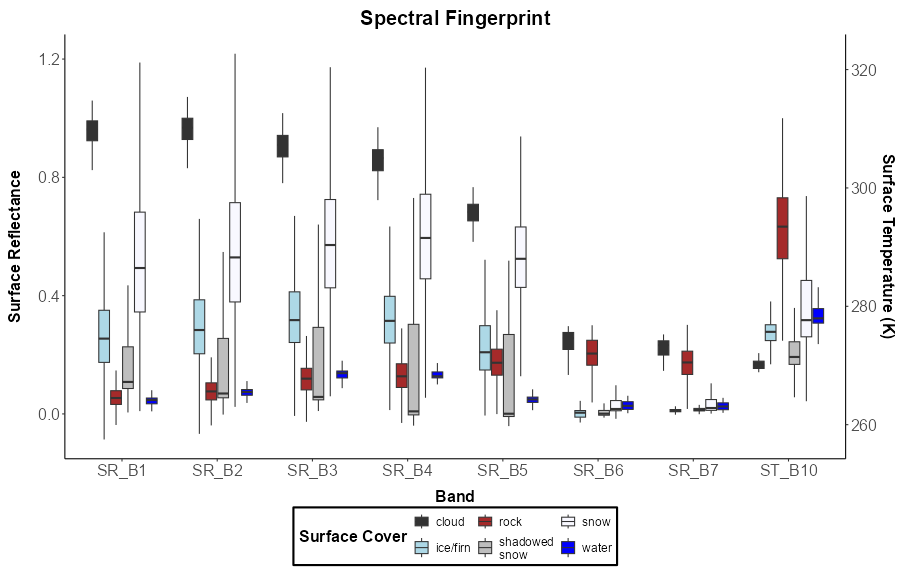
\includegraphics[keepaspectratio]{images/SpectralFingerprint_SR_ST.png}}

}

\caption{\label{fig-fingerprint-SR}The spectral fingerprint of surface
reflectance and surface temperature for Landsat 8/9 images across 6
surface cover classes ``cloud'', ``ice/firn'', ``rock'', ``shadowed
snow'', ``snow'', and ``water''.}

\end{figure}%

\begin{figure}

\centering{

\pandocbounded{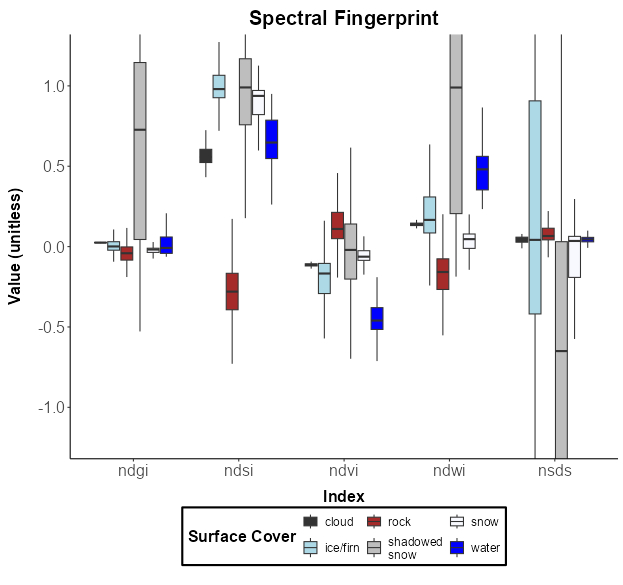
\includegraphics[keepaspectratio]{images/SpectralFingerprint_Indicies.png}}

}

\caption{\label{fig-fingerprint-indeices}The spectral fingerprint of
five calculated indices, Normalized Difference Snow Index (NDSI),
Normalized Difference Glacier Index (NDGI), Normalized Difference Water
Index (NDWI), Normalized SWIR Difference Soil-moisture (NSDS), and
Normalized Difference Vegetation Index (NDVI) from Landsat 8/9 images
across 6 surface cover classes ``cloud'', ``ice/firn'', ``rock'',
``shadowed snow'', ``snow'', and ``water''.}

\end{figure}%

For model training and testing a K-folds repeated cross-validation
method was utilized with 10 folds, 10 repeats, and a partition (p) = 0.9
resulting in a 90/10 training/testing split, where all labeled data
points are utilized in testing for exactly 1 of 10 folds/repeats. Using
this training/testing framework a total of 129 distinct ML models were
tested, across 10 model types, using a hyper-parameter grid search
performed in R utilizing the caret package (Kuhn, 2008). Based on the
accuracy results of this training/testing model optimization process,
the three best performing models were selected for additional model
validation using previously unseen, spatially-temporally distant
validation data. The top three, best performing models were, random
forest, support vector machine (SVM) using a linear kernel, and SVM with
a radial kernel Table~\ref{tbl-hyperparams}.

\begin{longtable}[]{@{}llc@{}}
\caption{The hyperparameters and testing accuracy for the three best
performing machine learning models on k-folds training-testing
data.}\label{tbl-hyperparams}\tabularnewline
\toprule\noalign{}
Model & Parameters & Testing Accuracy (k-folds) \\
\midrule\noalign{}
\endfirsthead
\toprule\noalign{}
Model & Parameters & Testing Accuracy (k-folds) \\
\midrule\noalign{}
\endhead
\bottomrule\noalign{}
\endlastfoot
Random Forest & mtry = 6 & 0.98 \\
Support Vector Machine & radial kernel; sigma = 1 and C = 8 & 0.98 \\
Support Vector Machine & linear kernel; C = 8 & 0.97 \\
\end{longtable}

Due to the spatial auto-correlation of the training/testing data,
K-folds methods are prone to over-inflating model accuracy with
geospatial datasets. Therefore, it is best practice to validate spatial
ML models using an additional dataset which is spatially-temporally
distant from the training/testing data and which has never been seen by
the model. In our study, we labeled 5,750 Greenland-specific validation
points for 5 locations, across 8 Landsat images. These locations were
chosen for validation to capture a range of regional variability across
the island. The five validation locations are, Mittivakkat glacier (3
dates/images), central-west peninsula (2), southern tip (1), Freya
glacier (central-east, 1), and far north (1). (Validation point locator
map figure).

\begin{figure}

\centering{

\pandocbounded{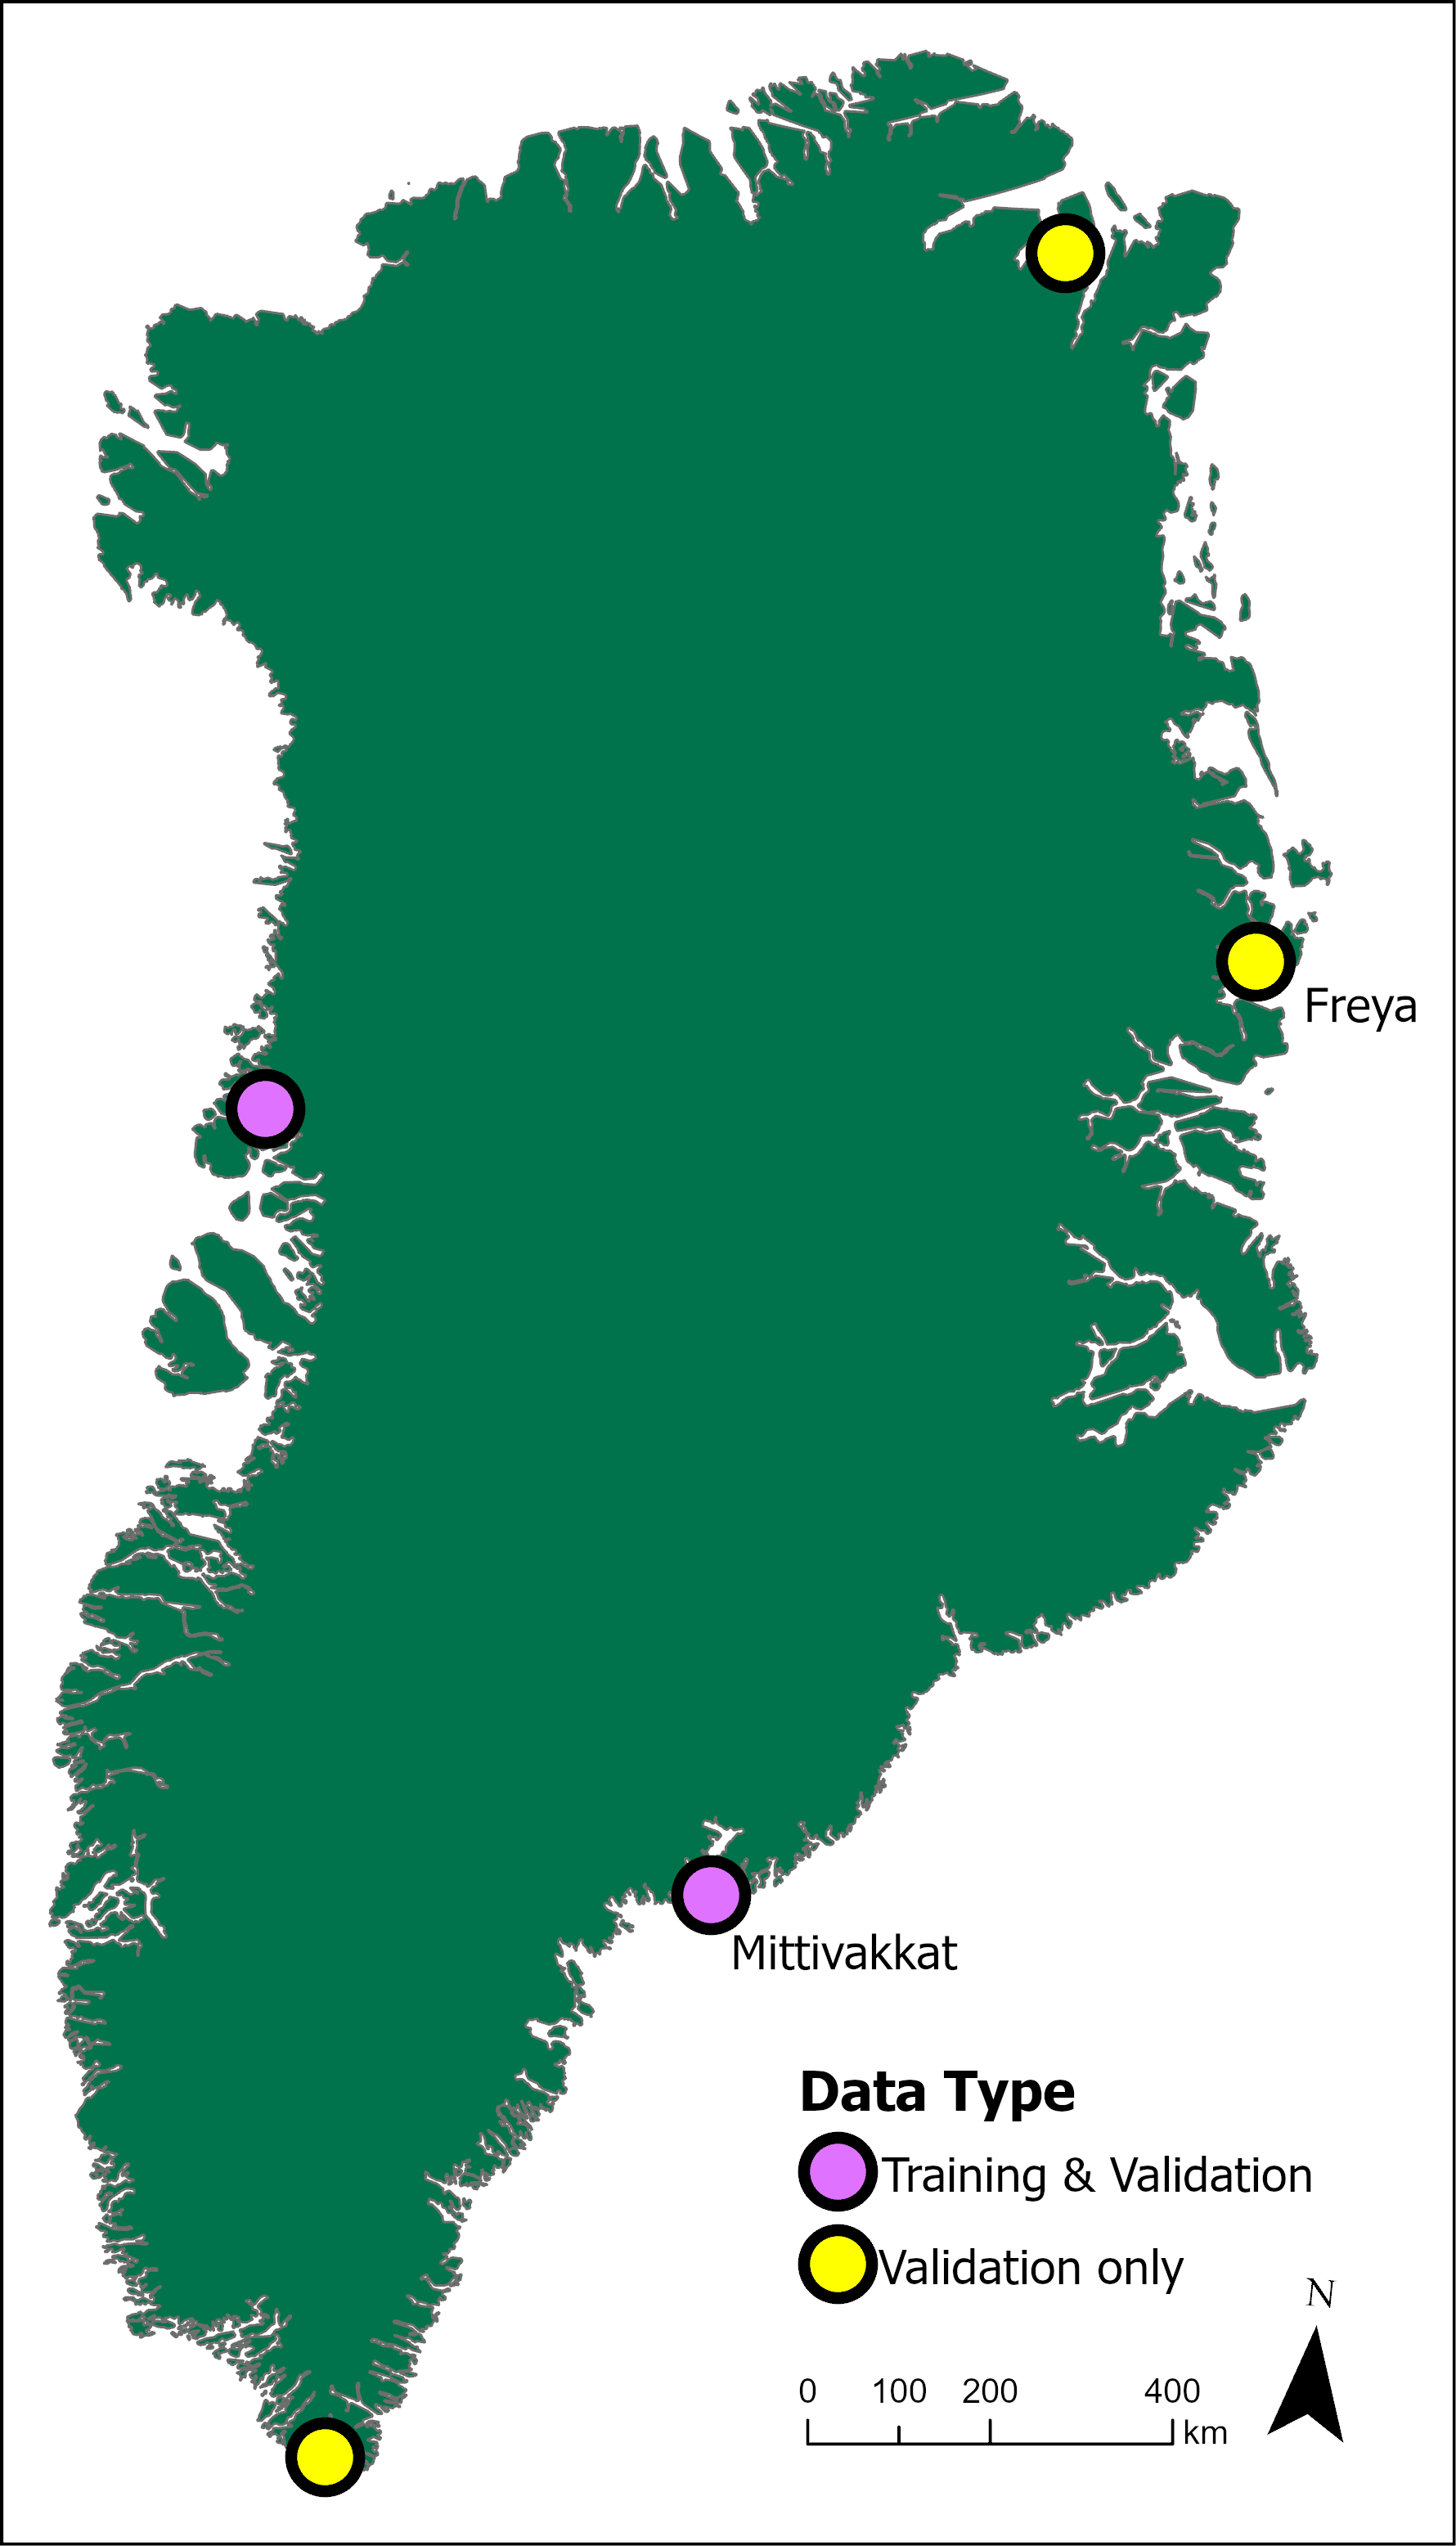
\includegraphics[keepaspectratio]{images/Training-Testing-Locator.png}}

}

\caption{\label{fig-training-location}Locations of training/testing and
validation datasets across Greenland. For locations with both training
and validation data the validation data was at least one year temporally
distant from the training data. World Glacier Monitoring Service
benchmark glaciers Mittivakkat and Freya labeled.}

\end{figure}%

The three best performing ML models were retrained using 100\% of the
available training data (10,812 labeled points) and were further
validated on previously unseen data. The overall accuracy of all models
decreased between 1-8\% from their prior K-folds accuracy, but
maintained a satisfactory ovrall accuracy. The best performing model on
the validation data was the SVM linear model, with an overall accuracy
of 93\% (Figure~\ref{fig-confusion}). The F1 statistic (a measure of
model performance) was 94\% for snow and 91\% for ice, the two most
critical classes for accurate Accumulation Area Ratio (AAR) calculation.

\begin{figure}

\centering{

\pandocbounded{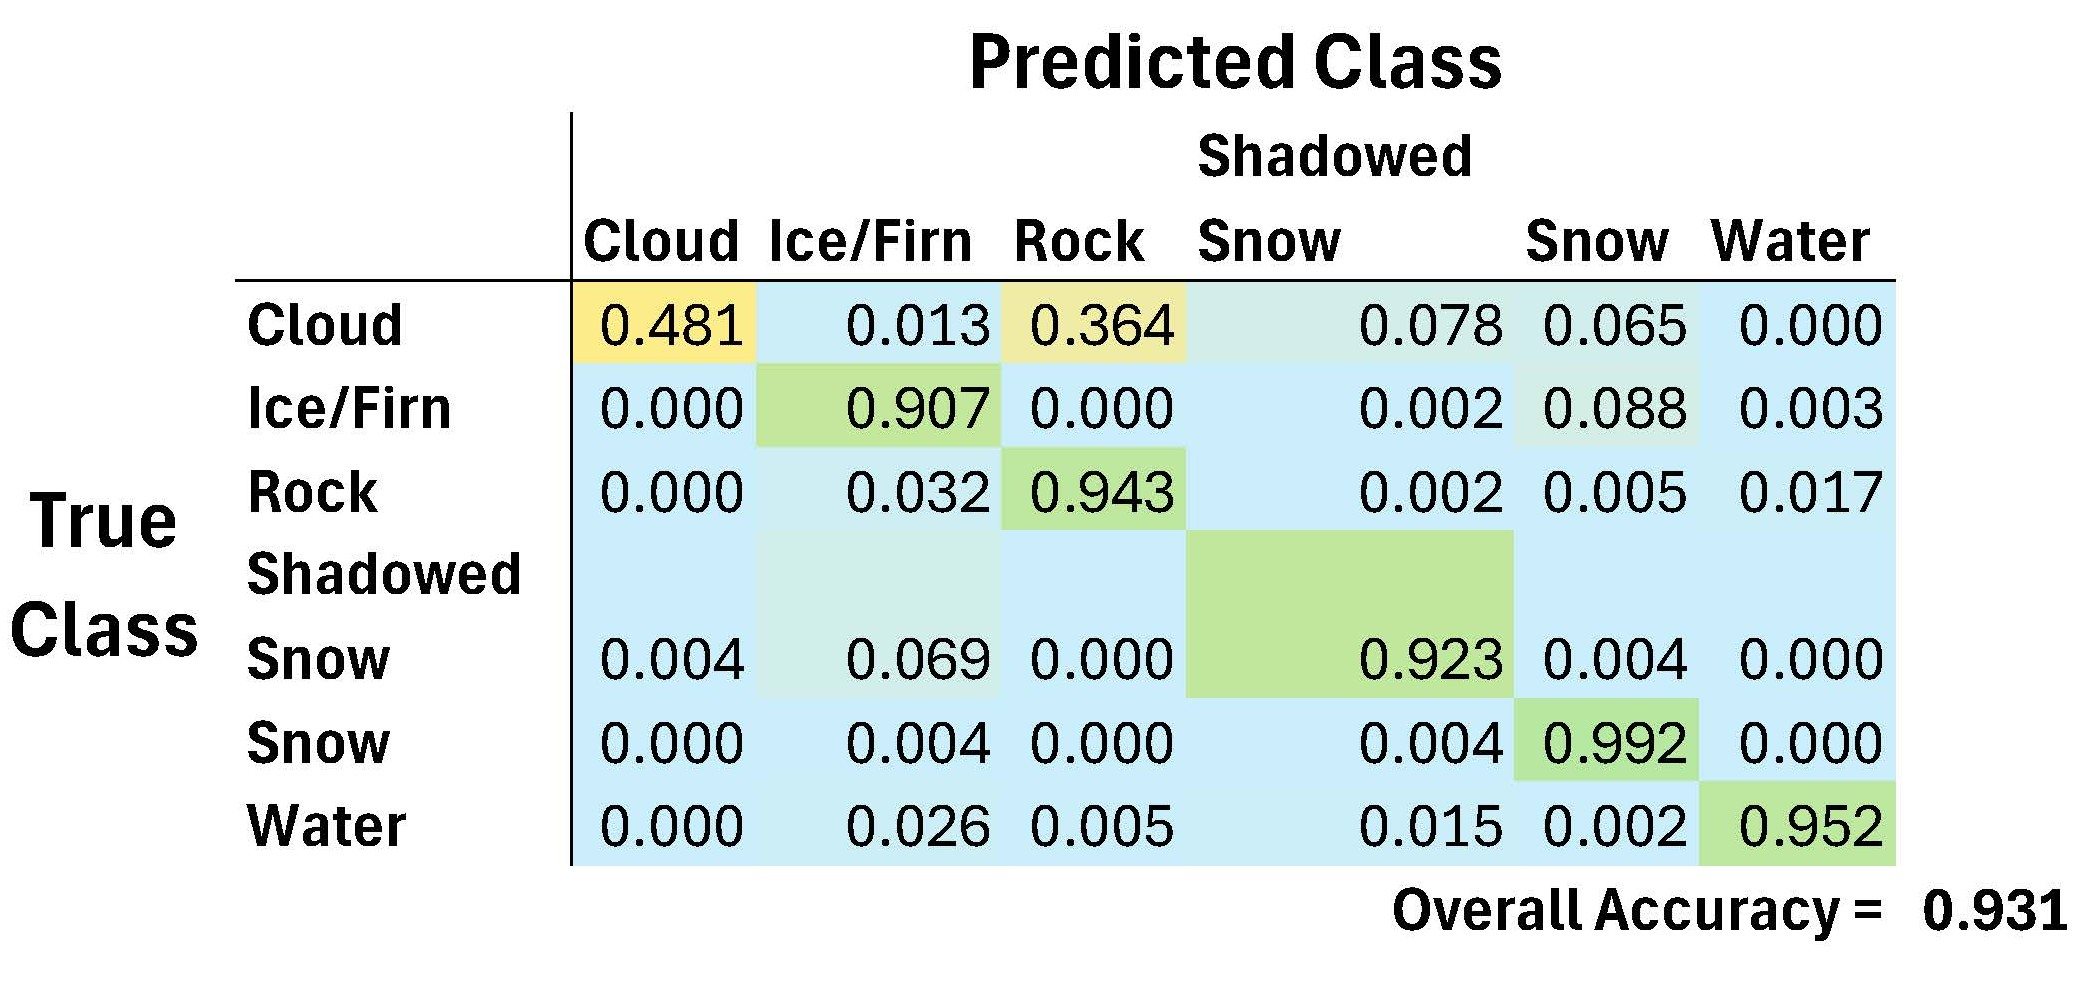
\includegraphics[keepaspectratio]{images/confusion-matrix-table.jpg}}

}

\caption{\label{fig-confusion}Glacier surface classification confusion
matrix for the validated surface vector machine learner with linerar
kernel across 6 surface cover classes, normalized as a frcation of total
validation points, color coded by accuracy.}

\end{figure}%

\subsection{Land Cover Classification}\label{sec-lcc}

\subsubsection{Data Acquisition}\label{sec-lcc-data}

Following model validation, all applicable Landsat 8 \& 9 Collection 2
Level-2, Tier 1 surface reflectance Science Products images from
2015-2025 during the ablation season (JJAS) which contained at least one
peripheral glacier were downloaded using either GEE geedim python
package or the United States Geological Survey (USGS) EarthExplorer data
portal. Images taken on ascending orbits, and images which only covered
the Greenland ice sheet but did not contain any peripheral glaciers were
excluded. In total, 20,562 unique images were downloaded
(\textasciitilde17 TB).

\subsubsection{Image Preprocessing and
Classification}\label{sec-classification}

Landsat images and the pretrained SVM model were uploaded to the
Arizona State University (ASU) Sol super computer (Sol) for processing
(Jennewein et al., 2023). Raw Landsat images were initially converted to
surface reflectance and surface temperature data using established
scaling factors for the OLI and TIRS instruments respectively. Images
were then masked to peripheral glaciers using a buffered version of the
Randolf Glacier Inventory (RGI) glacier outlines (RGI Consortium, 2023).
A secondary cloud mask was applied based on a modified version of the
Antarctic cloud mask developed by Moussavi et al. (2020). After masking,
the five indices were calculated as with the training dataset.

Preprocessed images were classified according to the pretrained SVM
(linear) model. For each classified image, glaciers with at least 70\%
classification coverage were identified by a spatial query with the
image extent. For each of the glaciers identified the surface area for
each landcover class was extracted from the classified image along with
relevant image metadata. For each glacier observation the transient AAR
was calculated according to equations \ref{eq-snow-area} to
\ref{eq-trans-aar}. Each glacier observation and associated calculations
was appended to a data file, culminating in \textasciitilde4.6 million
glacier observations. This data file was downloaded for further
post-processing.

\begin{equation}\phantomsection\label{eq-snow-area}{
Total\:Snow\:Area\:(km^2) = snow + shadowed\:snow
}\end{equation} \begin{equation}\phantomsection\label{eq-glacier-area}{
Total\:Glacier\:Area\:(km^2) = Total\:Snow\:Area + ice/firn
}\end{equation} \begin{equation}\phantomsection\label{eq-trans-aar}{
Transient\:AAR = \frac{Total\:Snow\:Area}{Total\:Glacier\:Area}
}\end{equation}

\subsection{Postprocessing}\label{sec-postprocessing}

Glacier observation data was postprocessed in R using the data.table
package for fast, efficient handling of large datasets (Barrett et al.,
2026; R Core Team, 2021). Spatial data was handled using the sf package
(Pebesma, 2018).

\subsubsection{Quality Control and Data Filtering}\label{sec-QC}

A variety of quality control and filtering steps were utilizedTo ensure
that appropriate annual (end-of-season) AAR values were identified from
the transient AAR dataset. First, glacier observations were filtered by
their calculated glacier area. Then they were filtered by cloud cover,
shadowed snow ratio, glacier size, glacier slope, and finally by date.

The first observation filtering process leveraged the glacier area to
identify and screen poorly classified images. The glacier area is
calculated according to Equation~\ref{eq-glacier-area}, and the glacier
area ratio is standardized by dividing the glacier area by its RGI
glacier extent (circa 2000). Ideally, throughout the ablation season,
the glacier area ratio is expected to vary smoothly from
\textasciitilde1 (spring; fully snow covered) to some minimum value
(late summer; exposed ice and rock near terminous), followed by a rapid
rebound (end of ablation; onset of seasonal snowfall). In practice a
combination of cloudy images and poor image classification can drive the
glacier area ratio down. To screen these poor quality images a loess
function was fit to the glacier area ratio data for each glacier-year.
The residuals were calculated for each glacier observation, and
observations with residuals \textless{} the 25\textsuperscript{th}
percentile per glacier-year were filtered out (Figure~\ref{fig-loess}).

\begin{figure}

\centering{

\pandocbounded{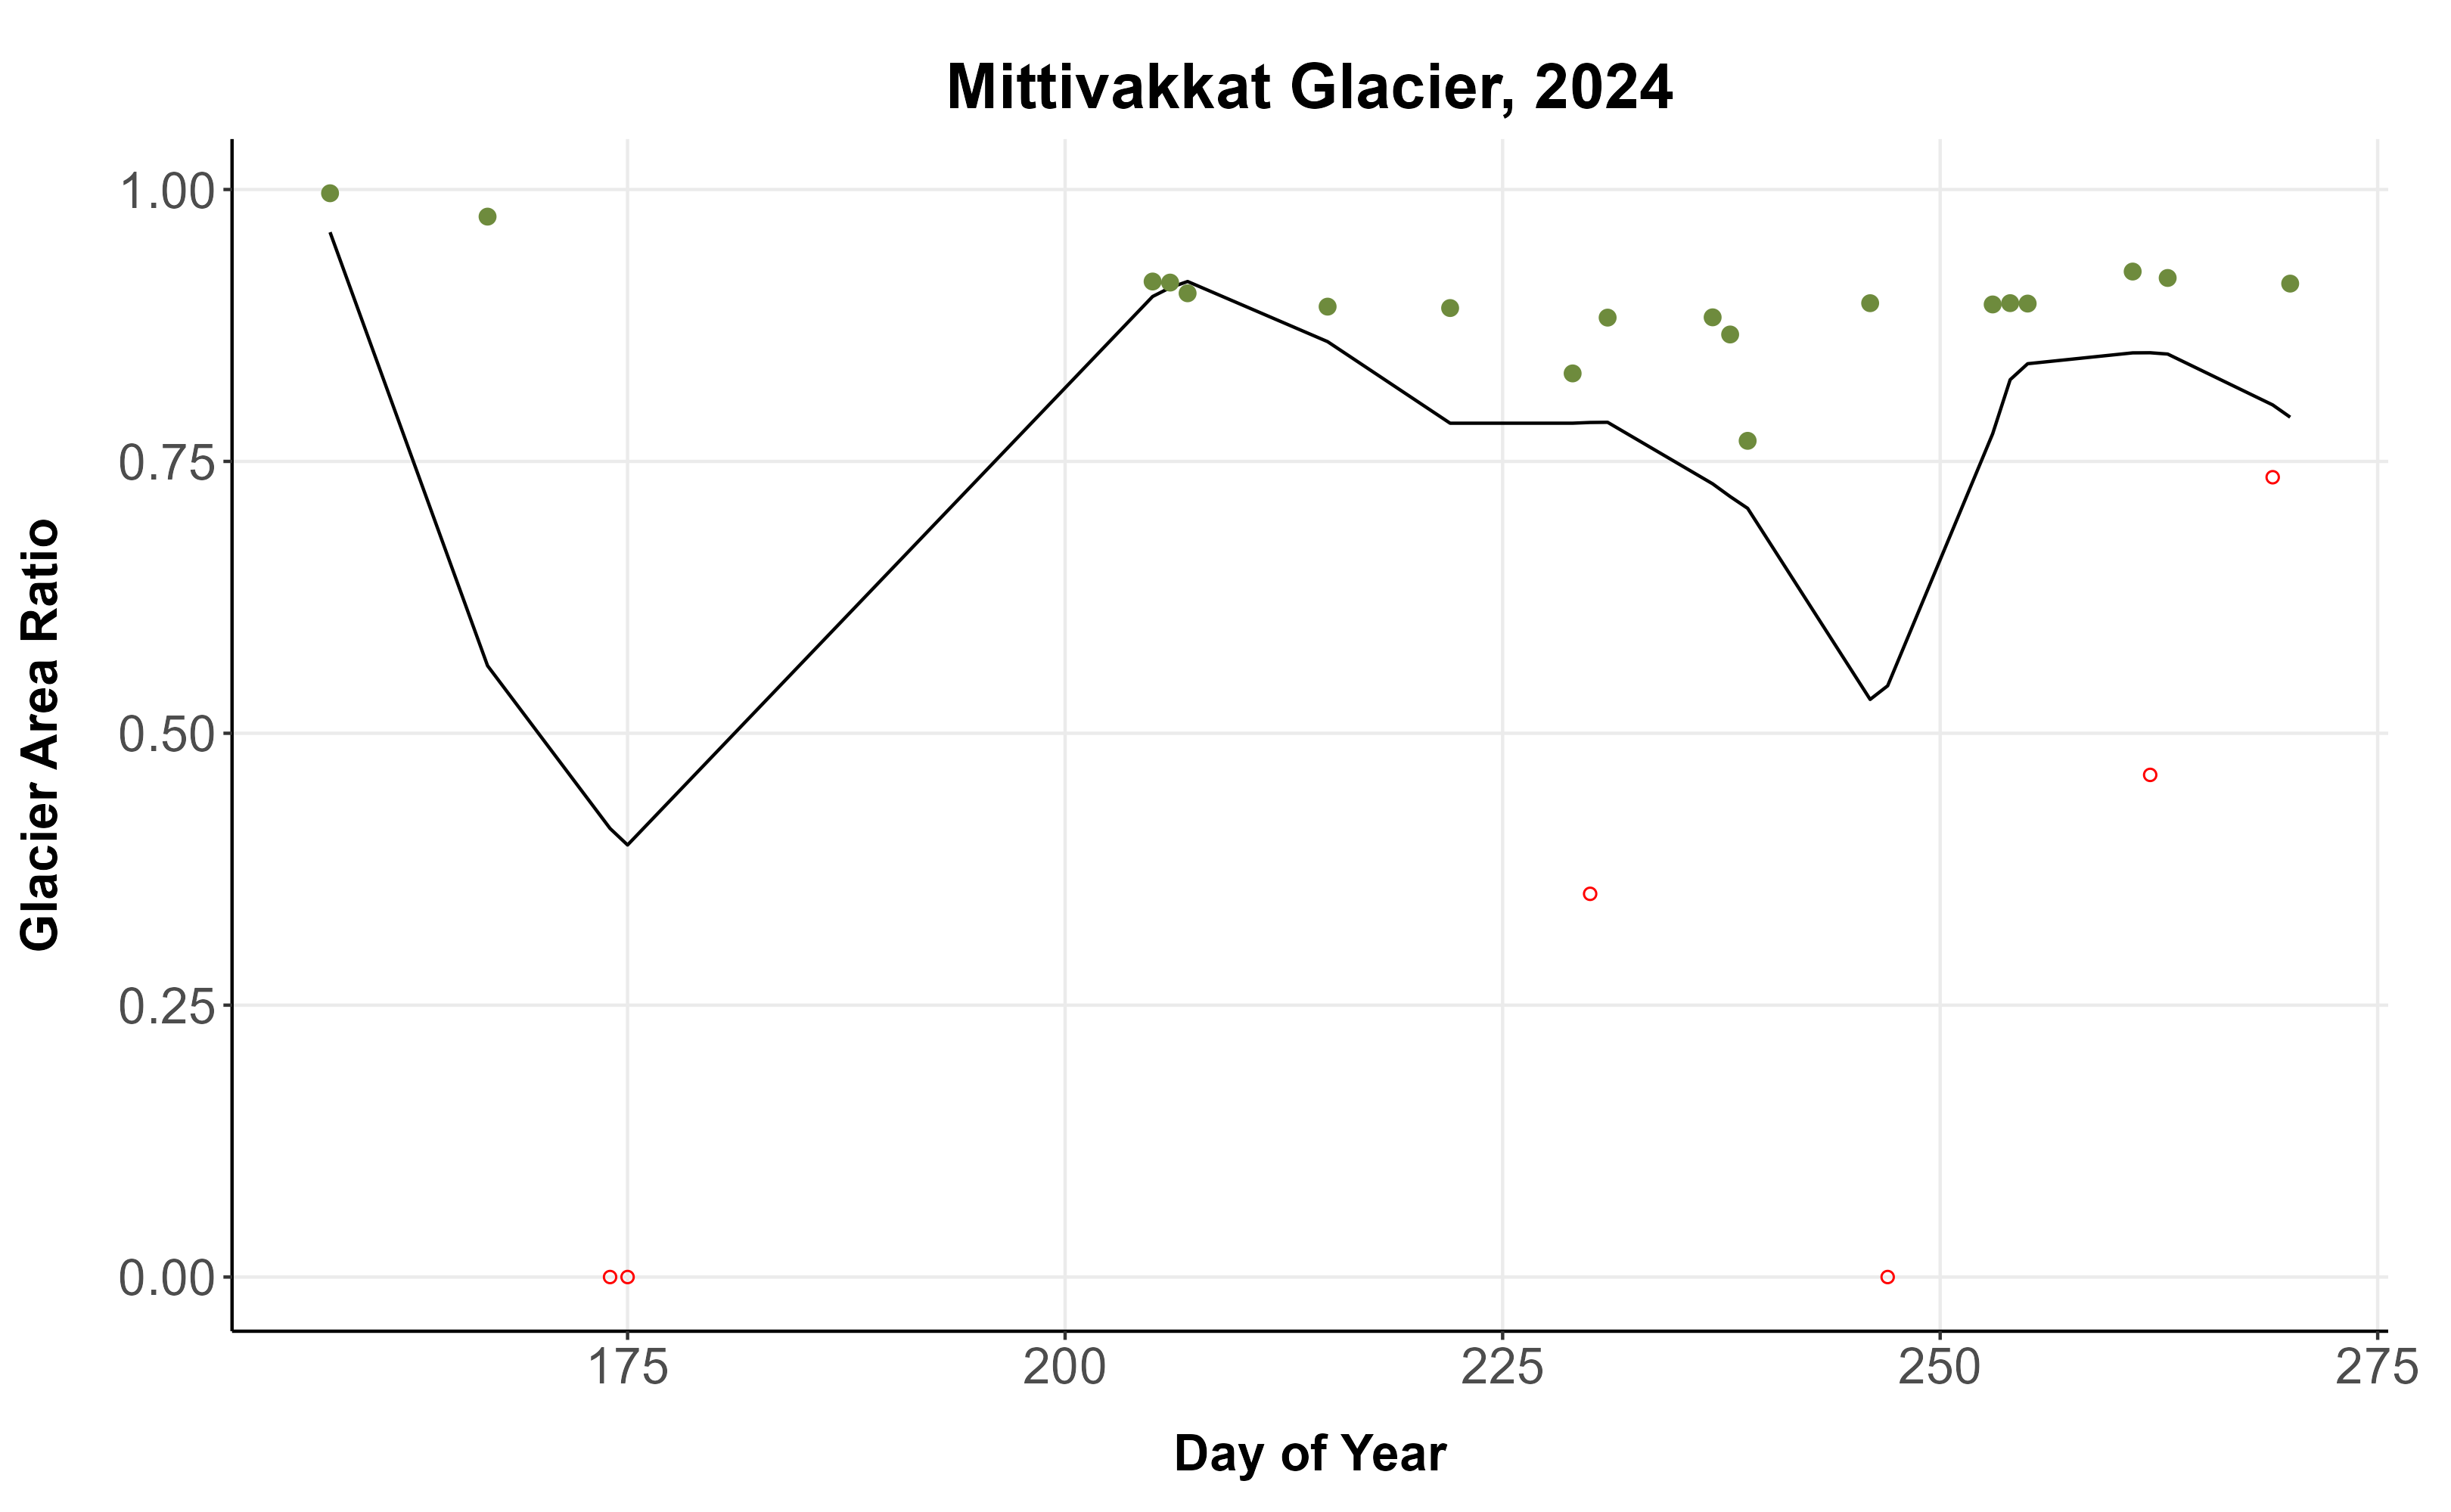
\includegraphics[keepaspectratio]{images/Mitt_2024_FAR_filter.png}}

}

\caption{\label{fig-loess}Graphical representation of the glacier area
ratio, glacier observation filtering process for Mittivakkat glacier,
2024. A loess smoothing function (black line) is fit to the dataset.
Glacier observations with a model residual \textless{} the
25\textsuperscript{th} percentile are removed (open red circles). All
other datapoints are retained (green points).}

\end{figure}%

Several additional simple filters were applied to the transient AAR data
according to AAR accuracy spot-checks and sensitivity analysis
Table~\ref{tbl-filters}. After all other filters were applied, the
number of remaining quality glacier observations were counted for each
glacier year. Glacier years which did not have at least 9 quality
observations were removed.

\begin{longtable}[]{@{}lll@{}}
\caption{Quality control filters applied to the transient AAR
dataset.}\label{tbl-filters}\tabularnewline
\toprule\noalign{}
Variable & Filter & Data Source/Equation \\
\midrule\noalign{}
\endfirsthead
\toprule\noalign{}
Variable & Filter & Data Source/Equation \\
\midrule\noalign{}
\endhead
\bottomrule\noalign{}
\endlastfoot
cloud cover & \textless{} 80\% & \(\frac{cloud\:area}{RGI\:area}\) \\
shadowed snow & \textless{} 50\% &
\(\frac{shadowed\:snow\:area}{RGI\:area}\) \\
glacier area & \textgreater{} 1 km\textsuperscript{2} \& \textless{} 300
km\textsuperscript{2} & RGI \\
slope & \textless{} 20° & RGI \\
day of year & \textless{} 259
(\textasciitilde Sep.~16\textsuperscript{th}) & Landsat image
metadata \\
n quality images & \textgreater{} 8 & filtered transient AAR data \\
\end{longtable}

\subsubsection{Annual AAR determination}\label{sec-aar}

From this filtered transient AAR dataset, the annual (end-of-season) AAR
was identified as the minimum remaining transient AAR value (hereafter,
AAR is synonymous with annual AAR). All late season glacier observations
occurring after the AAR date were filtered, and the number of remaining
glacier observations during the abblation period were counted. If a
glacier-year had at least 9 quality observations during the ablation
period (Section~\ref{sec-observation-density}), then the AAR was
considered valid, and the data was saved to a separate intermediate
datafile. In total 37,036 glacier-years had quality AAR data.

\subsubsection{Mean AAR}\label{sec-mean-aar}

The mean AAR (\(\overline{AAR}\)) was calculated as the arithmetic mean
of AAR for glaciers which had at least 5 years of quality data.
\(\overline{AAR}\) was saved to a separate datafile with 3,679 glaciers.

\subsection{Glacier-Year Observation Density Sensitivity
Analysis}\label{sec-observation-density}

To quantify the number of quality images needed for accurate
identification of the AAR, an observational density experiment was
performed. Twenty-one well-observed glacier-years were identified,
evenly distributed around Greenland, each with at least 30 quality
glacier observations (post filtering). For each glacier a series of
subseting experiments was performed where n randomly selected points
were subset from the glacier-year data. Using the randomly subset data,
the assumed AAR was selected and compared against the actual (known) AAR
from the full dataset. The n observations tested were; 3, 5, 7, 9, 12,
15, 20, 25, 30, and each experiment was repeated 100 times, for a total
of 18,900 simulations Figure~\ref{fig-obs-dense}. Based on the resultus
of these simulations, at least 9 quality observations per year are
needed to reliably identify the AAR Table~\ref{tbl-obs-dense}.

\begin{figure}

\centering{

\pandocbounded{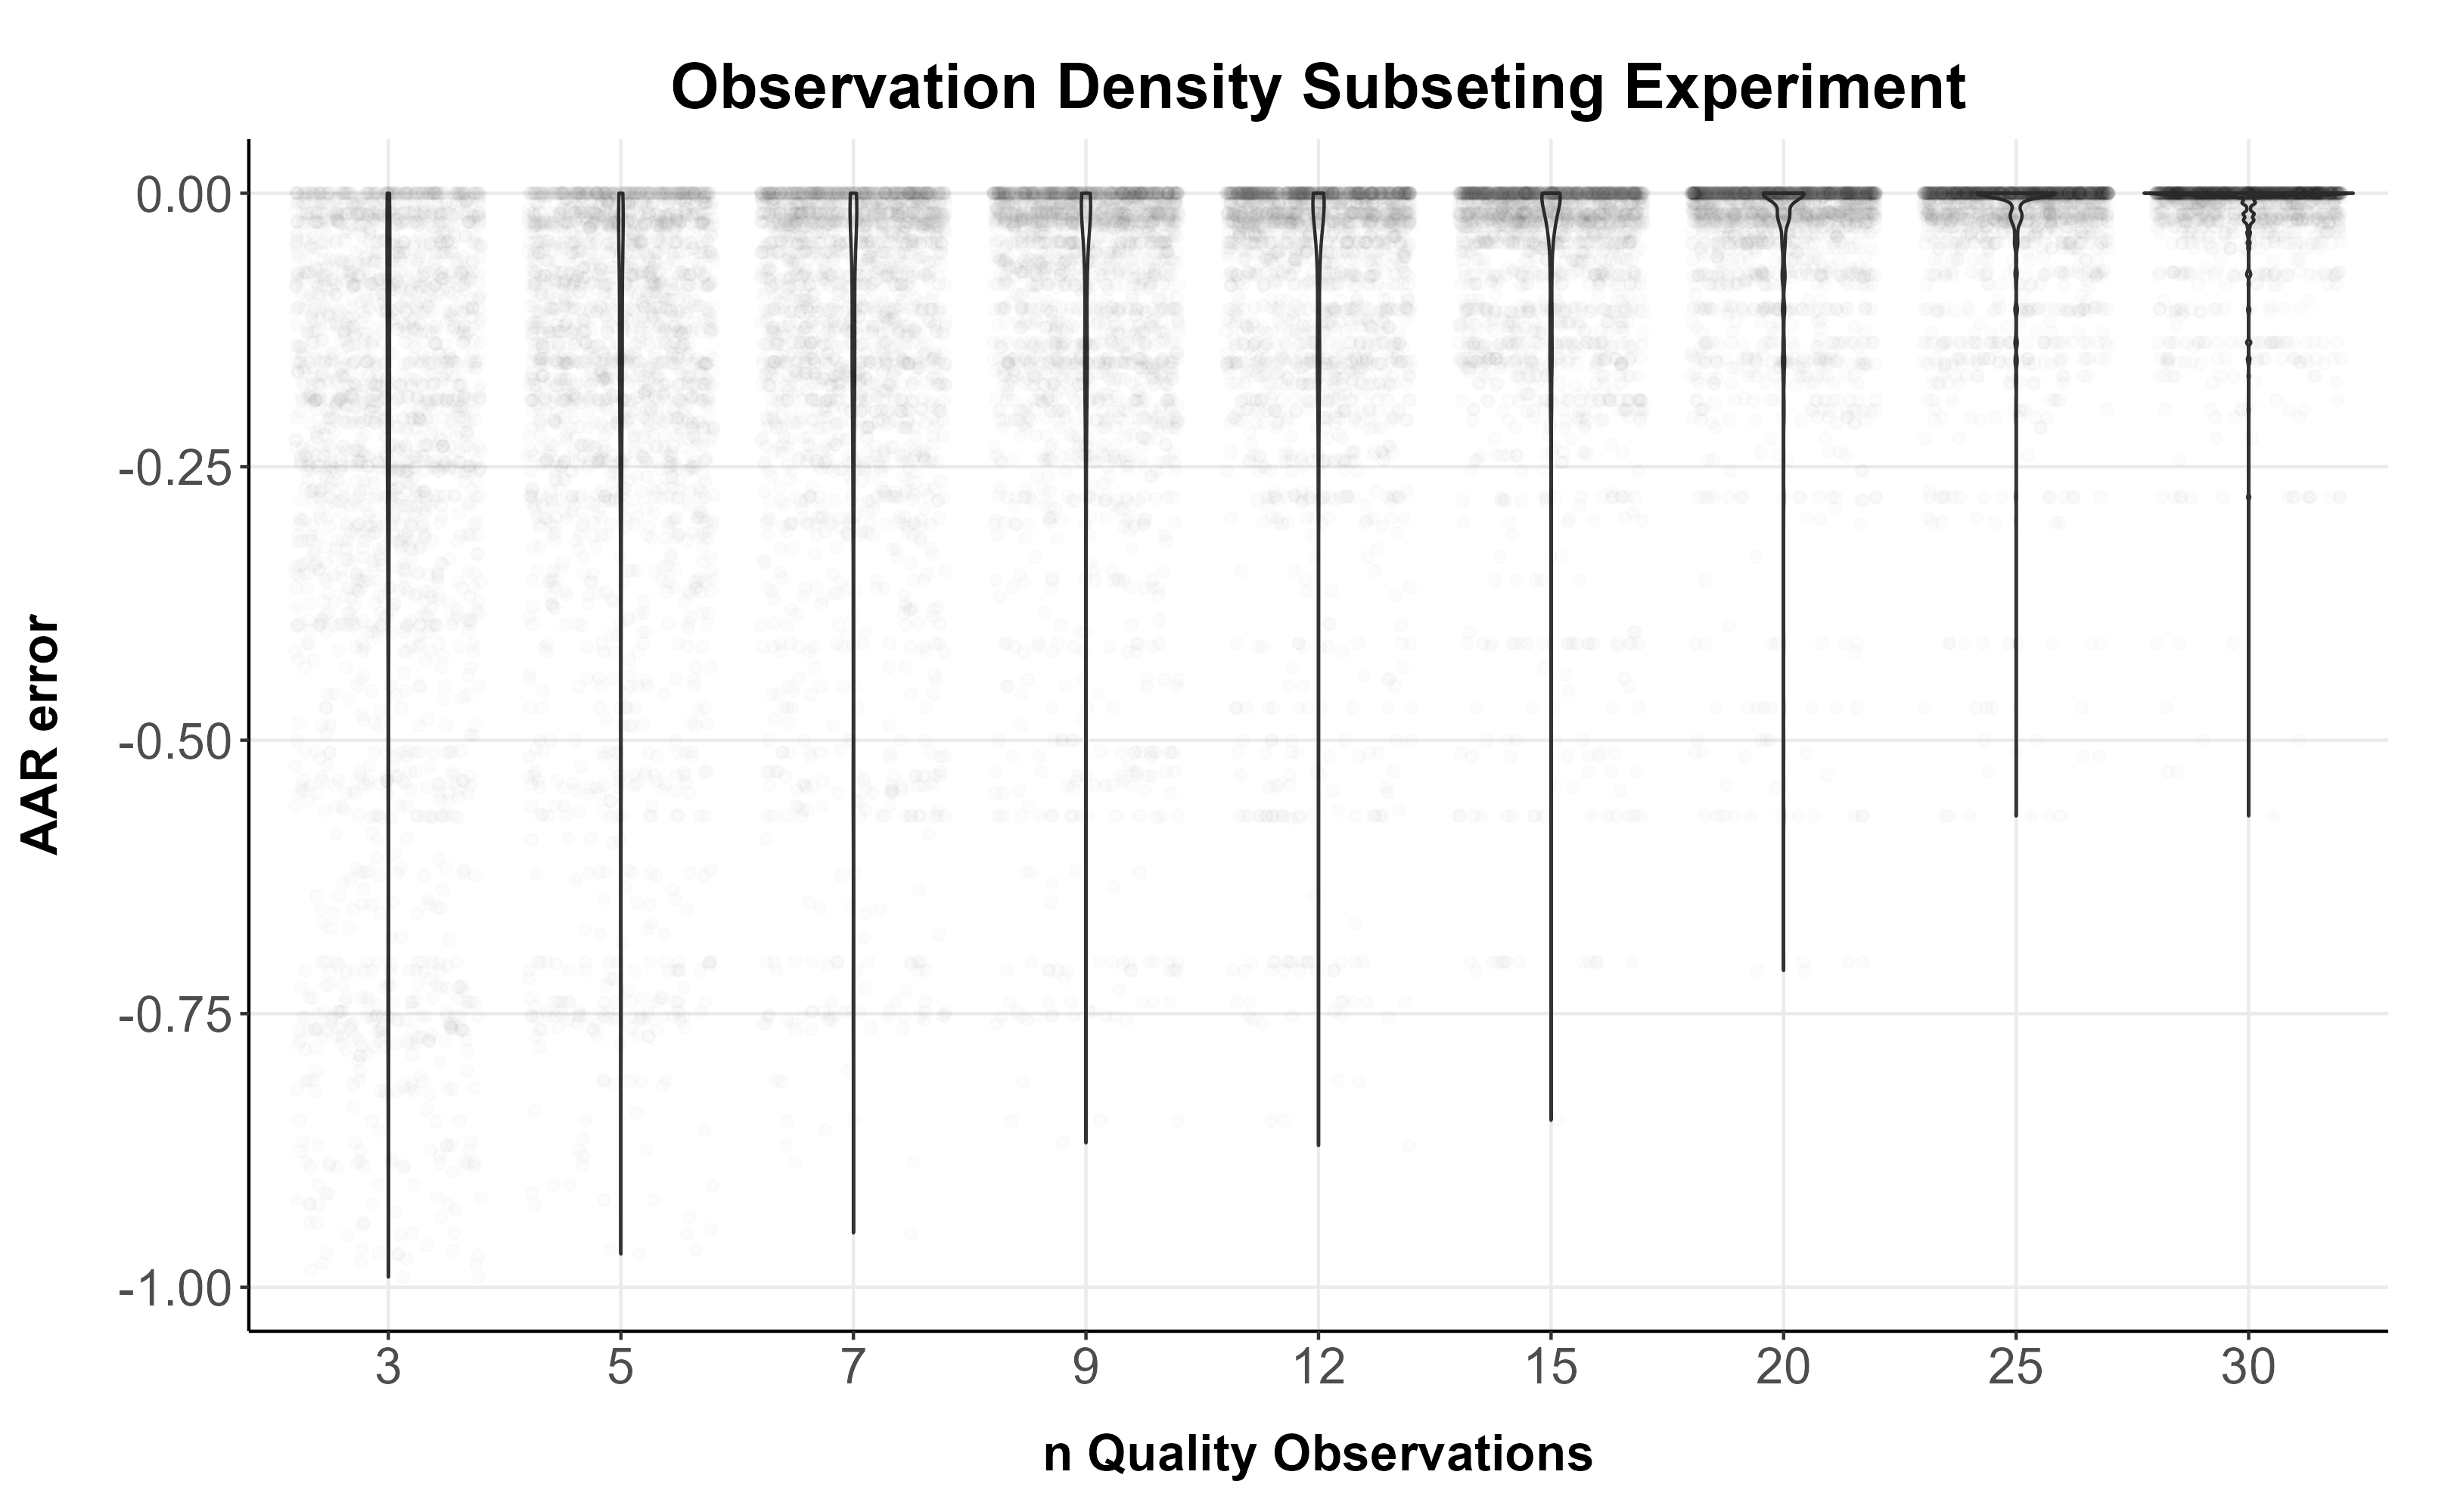
\includegraphics[keepaspectratio]{images/observation_density.png}}

}

\caption{\label{fig-obs-dense}Sensitivity of the AAR to the number of
quality observations in the dataset. Observations are randomly subset
from a selection of well observed glacier-years with at least 30 quality
observations. Violin plots and jittered scatterplot with partially
transparent points represent the density and variance of the
experimental AAR error relative to the known value.}

\end{figure}%

\begin{longtable}[]{@{}lrr@{}}
\caption{Mean and median AAR error rates for the observation density
sensitivity analysis (2,100 simulations per
subset).}\label{tbl-obs-dense}\tabularnewline
\toprule\noalign{}
n Quality Observations & mean AAR error & median AAR error \\
\midrule\noalign{}
\endfirsthead
\toprule\noalign{}
n Quality Observations & mean AAR error & median AAR error \\
\midrule\noalign{}
\endhead
\bottomrule\noalign{}
\endlastfoot
3 & -0.266 & -0.190 \\
5 & -0.188 & -0.126 \\
7 & -0.143 & -0.083 \\
9 & -0.114 & -0.045 \\
12 & -0.094 & -0.027 \\
15 & -0.067 & -0.019 \\
20 & -0.044 & -0.007 \\
25 & -0.030 & 0 \\
30 & -0.018 & 0 \\
\end{longtable}

\subsection{Equilibrium AAR and Committed Area Loss}\label{sec-aar0}

Equilibrium AAR (AAR\textsubscript{0}) values were given by Yang et al.
(2026). Disequalibrium (\(\alpha\)) and committed area loss
(\(\Delta\)A) were calculated according to Box et al. (2022). The
\(\Delta\)A values varried considerably by region, with the
central east (CE), north east (NE), south west (SW) all showing positive
committed area change (i.e., committed growth). Furthermore, while the
resulting \(\Delta\)A values are approximately centered on 0 (median =
-0.26 km\textsuperscript{2}) the distribution is not normal
(Figure~\ref{fig-delta-a-dist}). Rather, the distribution is highly
leptokurtic, with a slight positive skew. This indicates that, while
most glaciers are near their predicted equilibrium value, the
distribution is highly dominated by outliers on either side.

\begin{figure}

\centering{

\pandocbounded{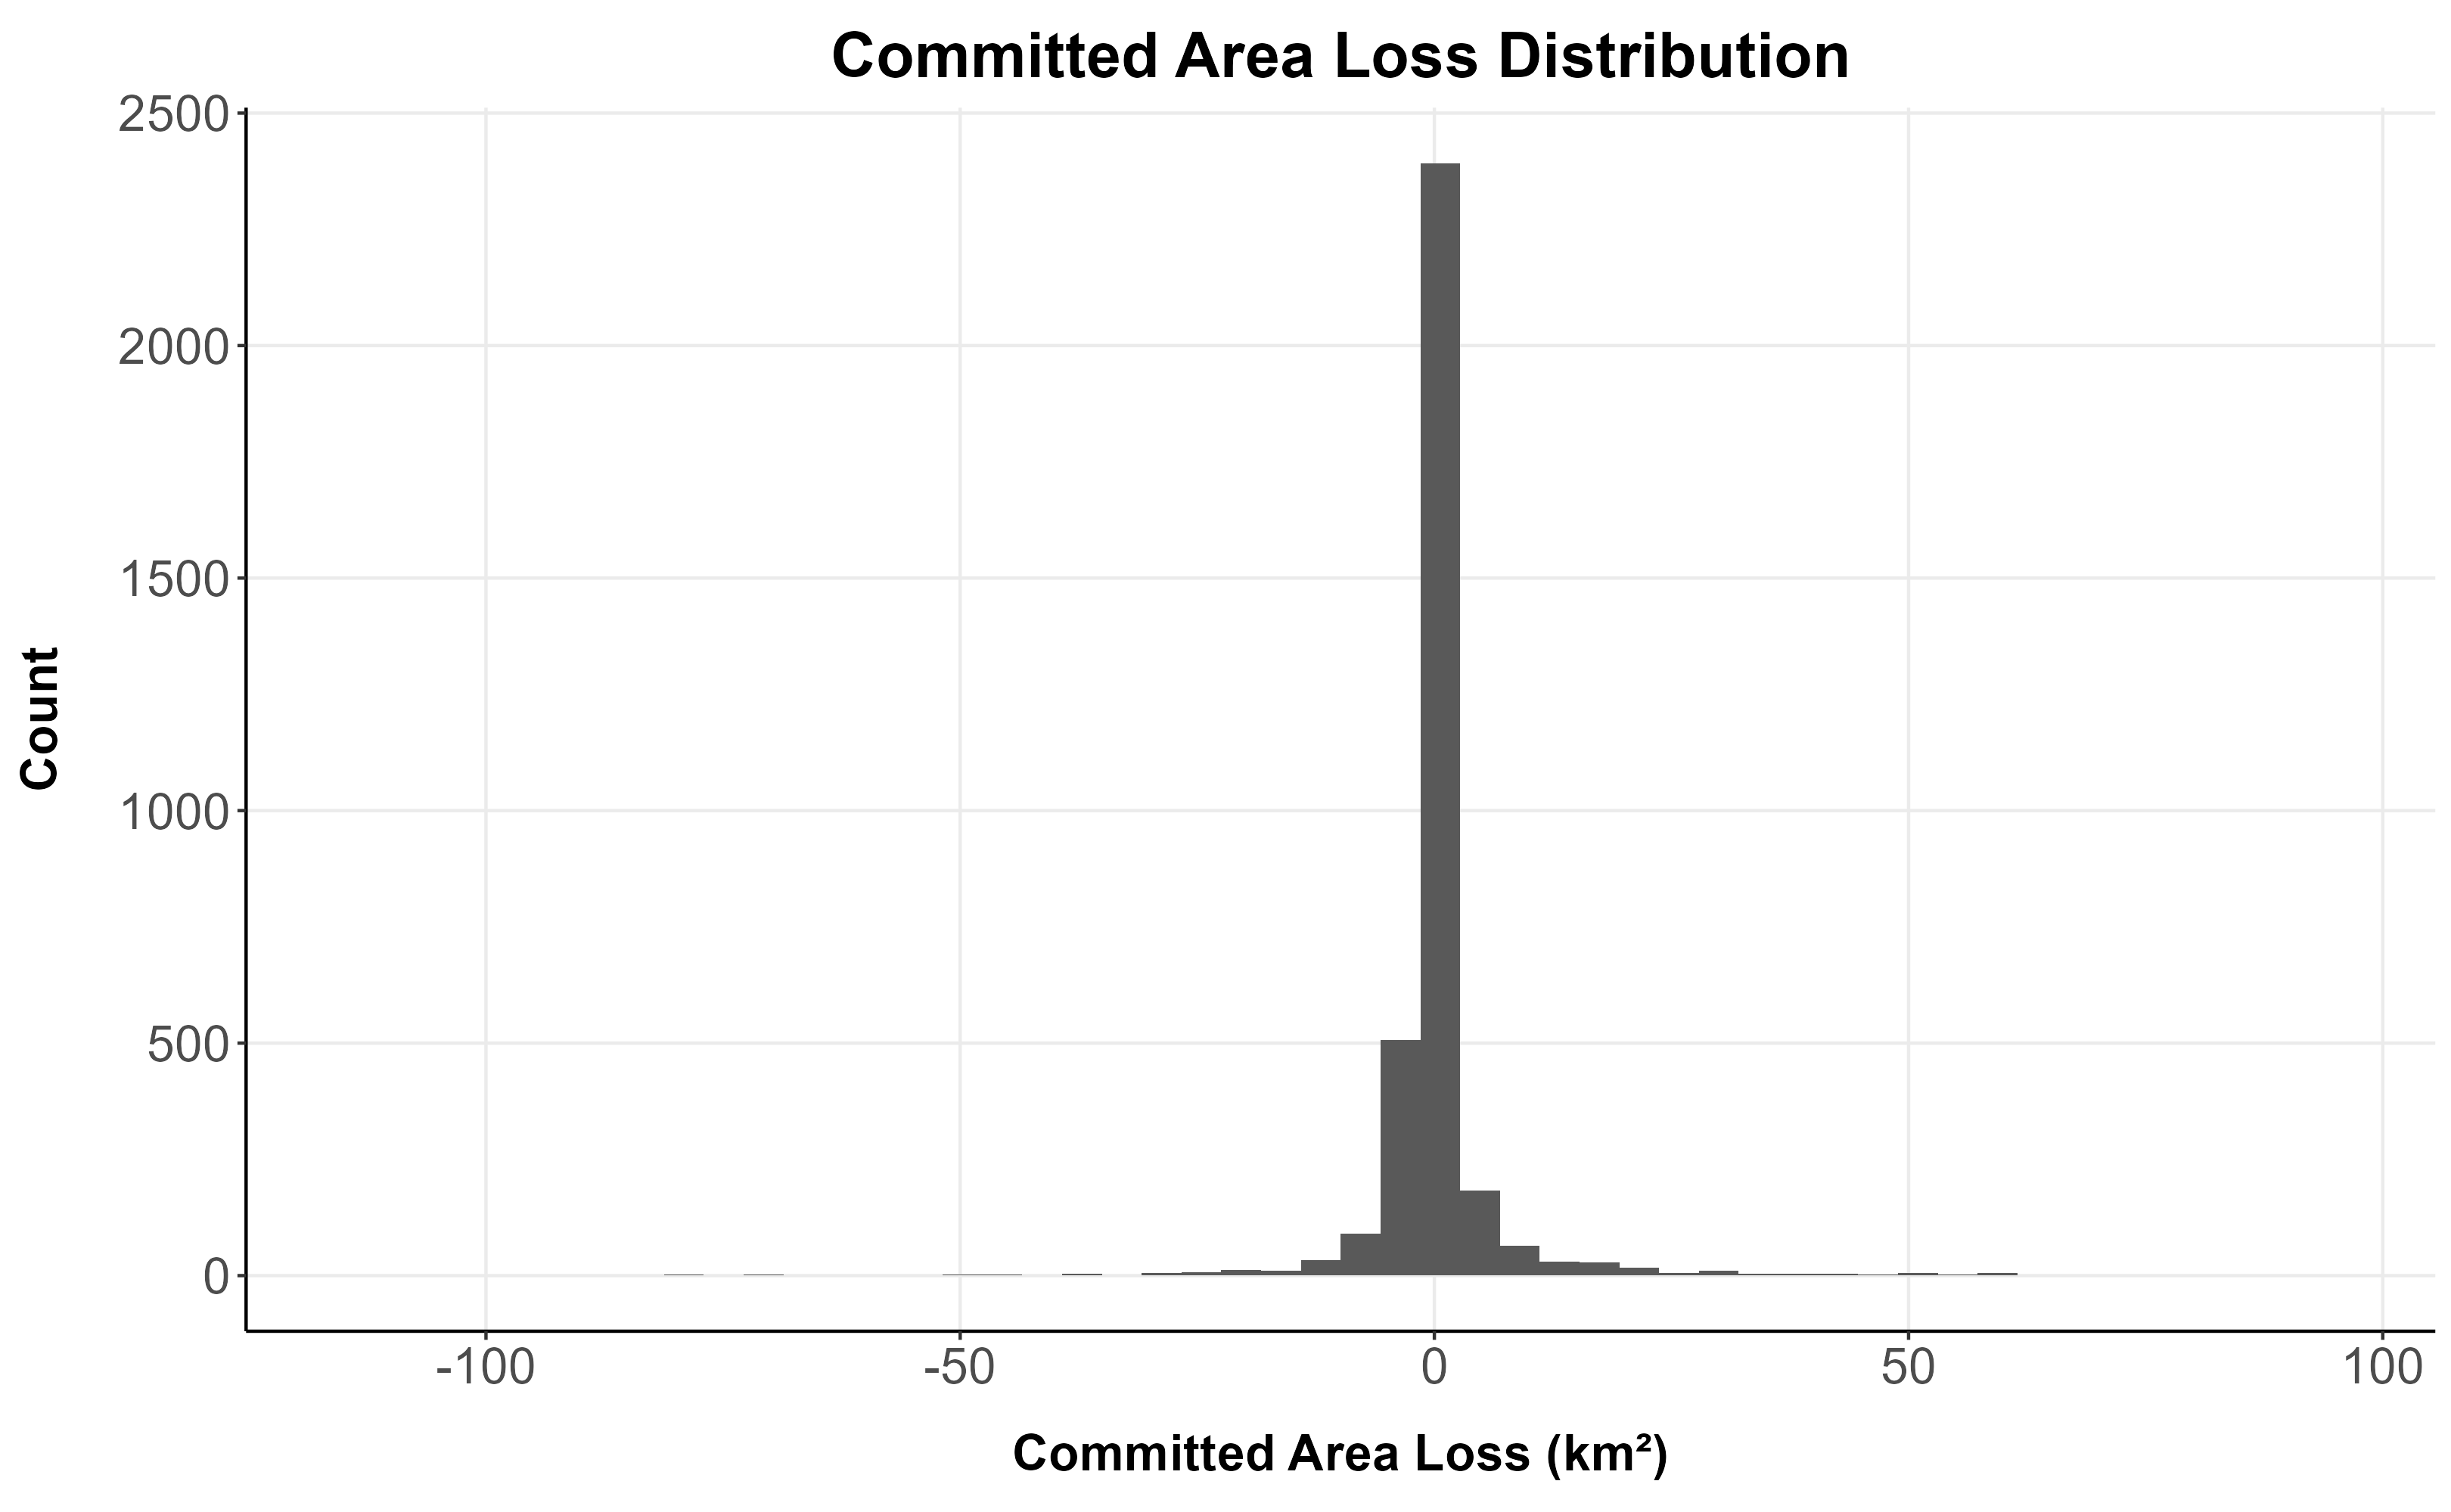
\includegraphics[keepaspectratio]{images/delta_A_dist.png}}

}

\caption{\label{fig-delta-a-dist}The highly leptokurtic distribution of
committed area change calculated using AAR\textsubscript{0} values by
Yang et al. (2026)}

\end{figure}%

\subsubsection{Committed Area Loss Sensitivity
Analysis}\label{sec-delta-a-sensitivity}

To further investigate the \(\Delta\)A results we conducted a
sensitivity analysis for a range of plausible AAR\textsubscript{0}
values, from 0.5 to 0.8, for each region individually as well as for
Greenland as a whole (Figure~\ref{fig-delta-a-sensitivity}). While most
regions exhibited relatively low sensitivity to AAR\textsubscript{0}
values, the NE and CE were both highly sensitive to a wide range of
AAR\textsubscript{0} values. Additionally, the SW was moderatly
sensitive to AAR\textsubscript{0} values between 0.5 and 0.6.
Importantly, these are also the three regions which are indicating
potential glacier growth. Therefore, small differences in either
\(\overline{AAR}\) or AAR\textsubscript{0} in any of these regions would
result in relatively large changes to \(\Delta\)A. Additionally, while
the CE continues to show positive \(\Delta\)A values up to
AAR\textsubscript{0} ≈ 0.68, the \(\Delta\)A for the NE crossess 0 at
AAR\textsubscript{0} ≈ 0.58 a difference of just 0.02 relative to the
Yang et al. (2026) data.

\begin{figure}

\centering{

\pandocbounded{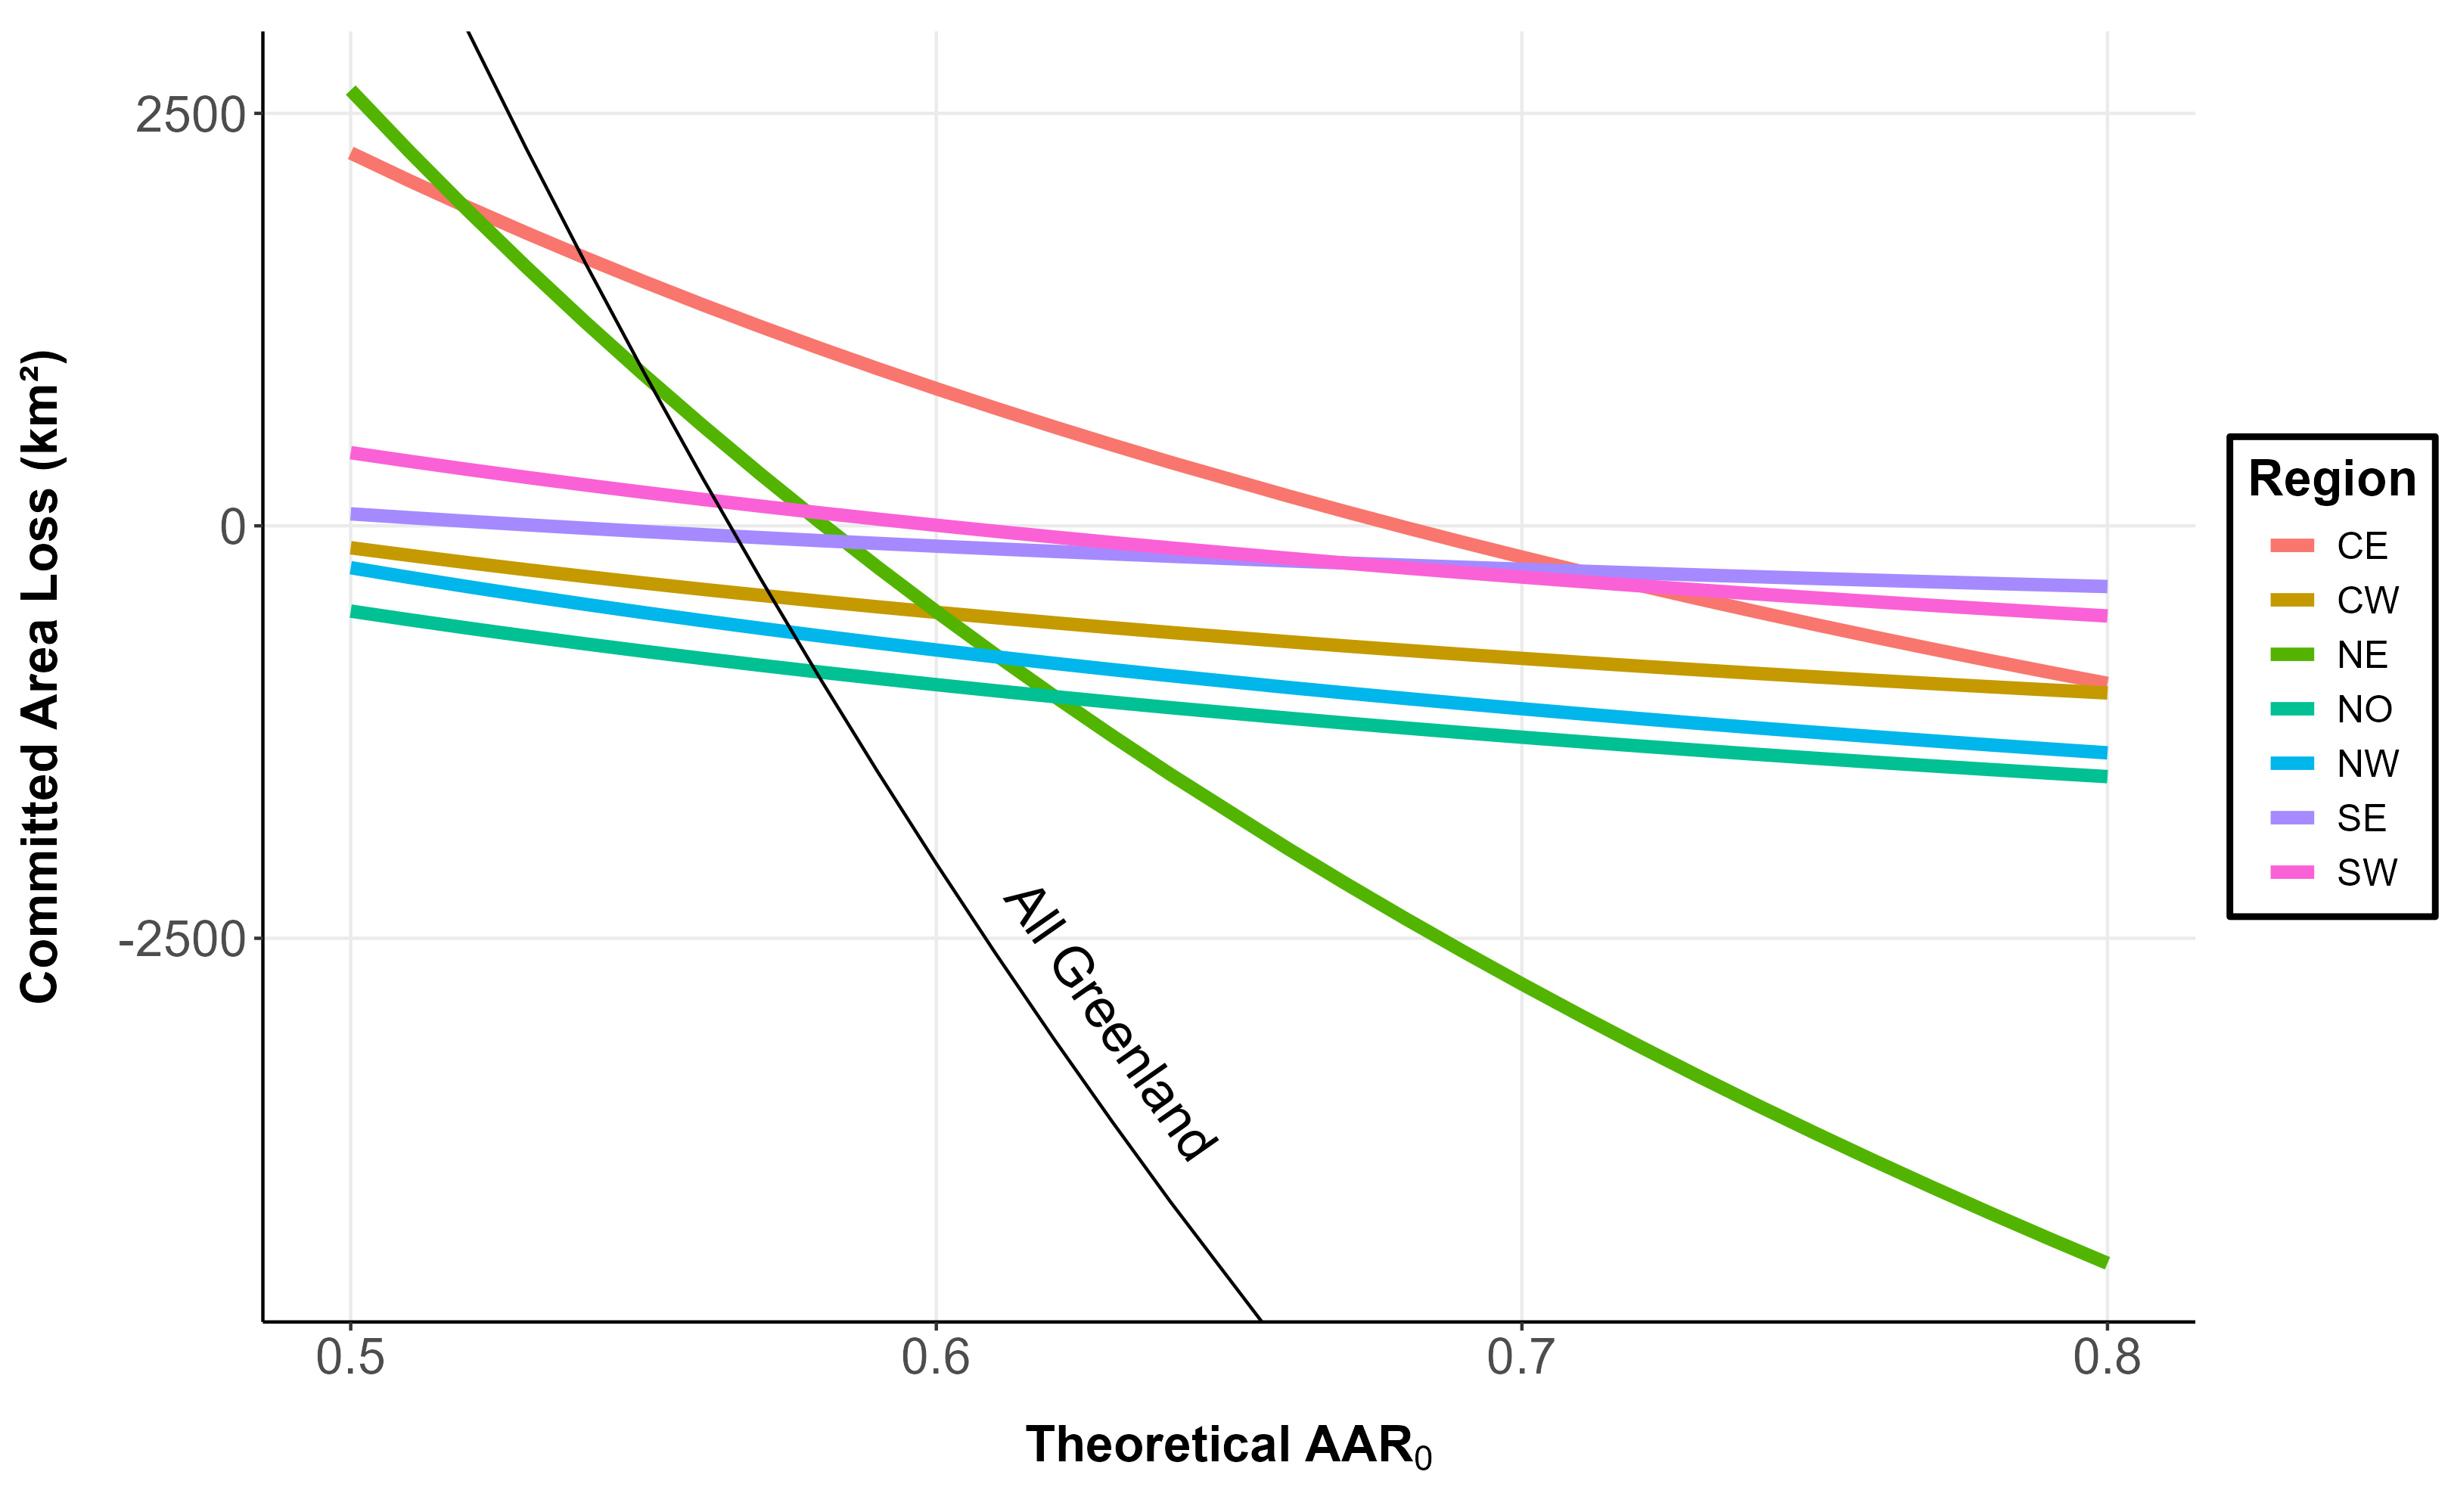
\includegraphics[keepaspectratio]{images/delta_A_sensitivity.png}}

}

\caption{\label{fig-delta-a-sensitivity}Sensitivity of committed area
loss to a range of plausible equilibrium AAR values. Thick lines color
coded by region, thin black line for all Greenland. Steeper lines
indicate greater sensitivity.}

\end{figure}%

\subsubsection{Review of Yang et al.~Methods and Accuracy within
Greenland}\label{review-of-yang-et-al.-methods-and-accuracy-within-greenland}

While the Yang et al. (2026) data is laudible, and on of the only
glacier-specific AAR\textsubscript{0} datasets available, it may not be
well suited for use in Greenland. For example, consider this large
glacier in the north west (NW) (RGI2000-v7.0-G-05-00250;
Figure~\ref{fig-glacier}). This glacier is the most extreme example of a
positive \(\Delta\)A in the dataset. With an \(\overline{AAR}\) of 0.63
and a realized area loss of \textless{} 2\% from circa 2020 to 2025 this
glacier appears to be relatively healthy. However, the Yang et al.
(2026) data lists the AAR\textsubscript{0} for this glacier as 0.45, a
shockingly low estimate. In fact, of the top 10 most positive
\(\Delta\)A glaciers in our data, 7 of them have AAR\textsubscript{0}
values \textless{} 0.5 (the losest tested theoretical
AAR\textsubscript{0} value in our sensitivity analysis). With global
paleio-climate AAR\textsubscript{0} estimates typically approximated at
0.58, values below 0.5 are quite low. Additionally, ice caps typically
have larger AAR\textsubscript{0} values, relative to equivalent mountain
glaciers.

\begin{figure}

\centering{

\pandocbounded{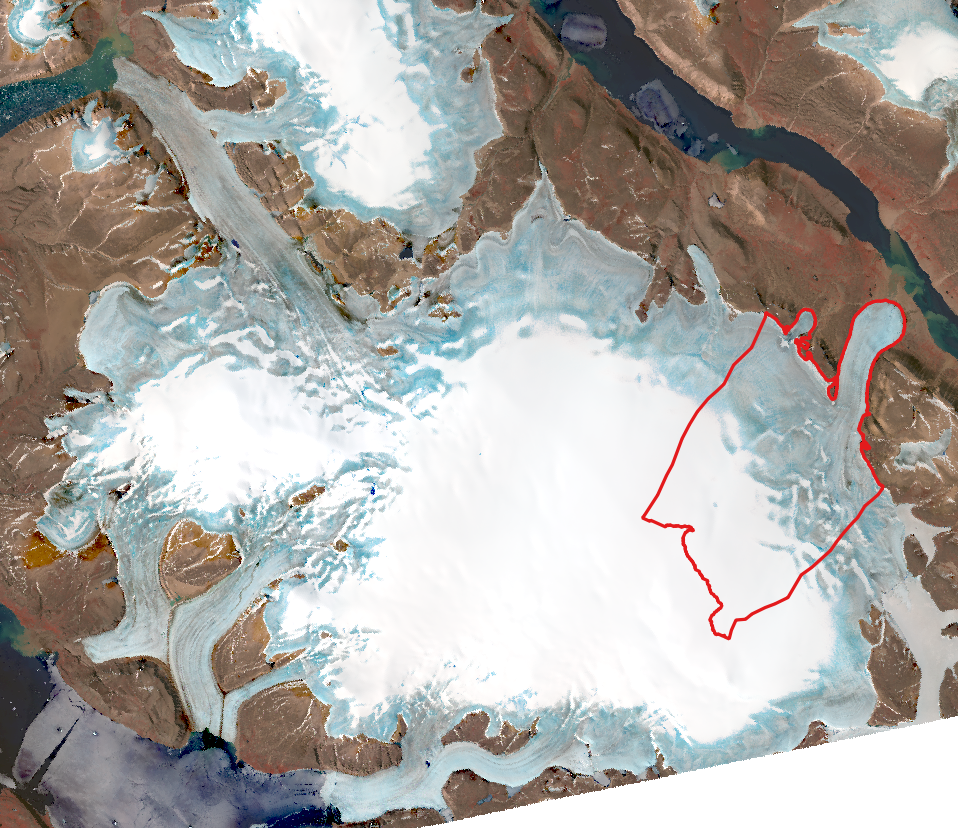
\includegraphics[keepaspectratio]{images/Yang_example.png}}

}

\caption{\label{fig-glacier}Glacier RGI2000-v7.0-G-05-00250 located in
the NW, part of a larger ice cap.}

\end{figure}%

These results call into question the accuracy of the Yang et al. (2026)
data within Greenland. Despite these concerns, it is not clear if the
Yang et al. (2026) is any more or less accurate than alternate
AAR\textsubscript{0} estimates, including global paleoclimate estimates.
Therefore, we present \(\Delta\)A values preliminaraly.

\section*{References}\label{references}
\addcontentsline{toc}{section}{References}

\phantomsection\label{refs}
\begin{CSLReferences}{1}{0}
\vspace{1em}

\bibitem[\citeproctext]{ref-Aberle_Enderlin_2025}
Aberle, R., Enderlin, E., O'Neel, S., Florentine, C., Sass, L., Dickson,
A., et al. (2025). Automated snow cover detection on mountain glaciers
using spaceborne imagery and machine learning. \emph{The Cryosphere},
\emph{19}(4), 1675--1693. \url{https://doi.org/10.5194/tc-19-1675-2025}

\bibitem[\citeproctext]{ref-data.table_2026}
Barrett, T., Dowle, M., Srinivasan, A., Gorecki, J., Chirico, M.,
Hocking, T., et al. (2026). \emph{Data.table: Extension of
`data.frame`}. Retrieved from \url{https://r-datatable.com}

\bibitem[\citeproctext]{ref-Box_Hubbard_2022}
Box, J. E., Hubbard, A., Bahr, D. B., Colgan, W. T., Fettweis, X.,
Mankoff, K. D., et al. (2022). Greenland ice sheet climate
disequilibrium and committed sea-level rise. \emph{Nature Climate
Change}, \emph{12}(9), 808--813.
\url{https://doi.org/10.1038/s41558-022-01441-2}

\bibitem[\citeproctext]{ref-HPC_2023}
Jennewein, D. M., Lee, J., Kurtz, C., Dizon, W., Shaeffer, I., Chapman,
A., et al. (2023). The sol supercomputer at arizona state university. In
\emph{Practice and experience in advanced research computing 2023:
Computing for the common good} (pp. 296--301). New York, NY, USA:
Association for Computing Machinery.
\url{https://doi.org/10.1145/3569951.3597573}

\bibitem[\citeproctext]{ref-Kuhn_2008}
Kuhn, M. (2008). Building predictive models in r using the caret
package. \emph{Journal of Statistical Software}, \emph{28}(5), 1--26.
\url{https://doi.org/10.18637/jss.v028.i05}

\bibitem[\citeproctext]{ref-Moussavi_2020}
Moussavi, M., Pope, A., Halberstadt, A. R. W., Trusel, L. D., Cioffi,
L., \& Abdalati, W. (2020). Antarctic supraglacial lake detection using
landsat 8 and sentinel-2 imagery: Towards continental generation of lake
volumes. \emph{Remote Sensing}, \emph{12}(1), 134.
\url{https://doi.org/10.3390/rs12010134}

\bibitem[\citeproctext]{ref-sf_2018-009}
Pebesma, E. (2018). The r journal: Simple features for r: Standardized
support for spatial vector data. \emph{The R Journal}, \emph{10},
439--446. \url{https://doi.org/10.32614/RJ-2018-009}

\bibitem[\citeproctext]{ref-R_2021}
R Core Team. (2021). \emph{R: A language and environment for statistical
computing}. Vienna, Austria: R Foundation for Statistical Computing.
Retrieved from \url{https://www.R-project.org/}

\bibitem[\citeproctext]{ref-RGI_2023}
RGI Consortium. (2023). Randolph glacier inventory - a dataset of global
glacier outlines, version 7. NASA National Snow; Ice Data Center
Distributed Active Archive Center.
\url{https://doi.org/10.5067/F6JMOVY5NAVZ}

\bibitem[\citeproctext]{ref-Yang_Mackintosh_2026}
Yang, W., Mackintosh, A. N., Cooper, E.-L., Li, Y., Jones, R. S., Chu,
W., \& Tielidze, L. G. (2026). Global estimates of glacier
equilibrium-line altitude ratios for enhanced paleoclimate
reconstructions. \emph{Communications Earth \& Environment}.
\url{https://doi.org/10.1038/s43247-026-03391-5}

\end{CSLReferences}




\end{document}
